%
% This template has been created by:
%   Pascal Bercher, 
%   - pascal.bercher@anu.edu.au, 
%   - https://bercher.net
%
% The newest version can be found on:
% https://gitlab.anu.edu.au/u1092535/latex-templates/
%
% Version number: 
%   Probably 1.08, but there's a chance it's actually
%   slightly newer and I just forgot to update this line. :)
%
% Version history:
%   Detailed change logs are provided in the file readme.txt.
%
% I was too lazy to put it under a specific license (will do
% so eventually; but might take me a few more years...), but
% you are still free to use and alter it. However, since I 
% put a *lot* of effort (and experience) in it, I insist on
% keeping my credentials in here (at the top), which give
% credit to me as an author. I explicitly forbid re-publishing
% my code (or content) until I put it under a specific license
% which would then clarify the rights. However, as said, *using*
% it is *of course* allowed, this is after all why I created it!
%
% Good luck with your thesis, and enjoy the journey  --  Pascal

\documentclass[a4paper,twoside,cleardoublepage=plain,bibliography=totoc]{scrbook}

\usepackage[a4paper]{geometry}                    % used for defining the title page

\usepackage{xurl}                                 % allows long URLs to break at any position
\usepackage[backref=page]{hyperref}               % defines style of references / links
\hypersetup{
linktocpage,                                      % in the table of contents, the numbers serve as links, not the entries
colorlinks  = true,                               % the items are colored instead of colored boxes around them
urlcolor    = cyan,
linkcolor   = red,
citecolor   = blue
}
% the following makes back references more appealing.
% Taken from: https://tex.stackexchange.com/questions/183702/formatting-back-references-in-bibliography-bibtex
\renewcommand*{\backref}[1]{}
\renewcommand*{\backrefalt}[4]{[%
\ifcase #1 Not cited.%
  \or Cited on page~#2.%
  \else Cited on pages #2.%
\fi]}




\usepackage{datetime}                                % to be able to print month & year on title page
  \newdateformat{monthonly}{\monthname[\THEMONTH]}
\usepackage{amssymb,amsthm,amsmath}                  % standard math packages; often used
\usepackage{graphicx}                                % allows including graphics
\usepackage{natbib}                                  % a specific citation style
\usepackage{floatrow}                                % allows to place a caption next to a figure
  \floatsetup[table]{capposition=top}                 % forces table captions to appear on top.
\usepackage[linesnumbered,ruled,vlined]{algorithm2e} % used for depicting algorithms
\usepackage{booktabs}                                % for tables that actually look nice!
\usepackage{paralist}                                % provides compactitem, a more compact itemize
\usepackage{titlesec}                                % used to add those horizontal lines around chapter package; see defs below.
\usepackage[standardsections]{scrhack}                % fixes an error causes by loading titlesec for class scrbook
\usepackage{parskip}                                 % when this is included, no indentations are used for new paragraphs,
                                                     % and instead paragraphs are separated by a small distance between them


% [requires titlesec]
% Surrounds all chapter titles by lines,
\titleformat{\chapter}[display]
{\bfseries\huge}
{\filleft\Large\chaptertitlename~\thechapter}
{3ex}
{\titlerule\vspace{1.5ex}\filright}
[\vspace{1ex}\titlerule]

% fixes a compilation errror that otherwise occurs in combination with scrbook
% see https://tex.stackexchange.com/questions/625083/adding-horizontal-line-before-and-after-chapter-heading-in-scrbook
% \titleformat{\section}
%  {\normalfont\Large\bfseries}{\thesection}{1em}{}
% \titleformat{\subsection}
%  {\normalfont\large\bfseries}{\thesubsection}{1em}{}
% \titleformat{\subsubsection}
%  {\normalfont\normalsize\bfseries}{\thesubsubsection}{1em}{}
 

 

% Set your individual data for the title page in the configuration file
% AND DON'T SCREW UP THIS DATA! You should know, for example, whether it's
% an Honours thesis or not, or in which semester it is running.

% Set your name:
%  (Well, your name.)
\newcommand{\AuthorName} {Pascal Bercher}


% Set the title of your work:
%  (Choose an informative and interesting title.)
\newcommand{\ProjectTitle} {Template for Project Reports}


% Set which titlepage layout you prefer. Both provide the exact same
% information, they only differ in design to give you a bit of individuality
%  (change second line accordingly)
\newif\ifStandardTitle % do not delete this part!
\StandardTitletrue     % comment out (or use \StandardTitlefalse)
                       % to switch to an alternative title page layout


% Set the name of your school:
%  (School of Computing, School of Engineering,
%   or School of Cybernetics)
\newcommand{\School} {School of Computing}


% Set the name of your college:
%  (However your College is called.)
\newcommand{\College} {College of Engineering, Computing and Cybernetics (CECC)}


% Set your project points:
%  (6 or 12)
%  can be ignored for Honours theses, since those are always 24 pt anyway
%  and hence set automatically
\newcommand{\ProjectPoints} {6}


% Set whether it's an Honours thesis:
%  (change second line accordingly)
\newif\ifHonoursThesis % do not delete this part!
\HonoursThesistrue     % or \HonoursThesisfalse or comment out


% Set your semester:
%  (S1 or S2 or S1/S2 or S2/S1 or Summer)
\newcommand{\Semester} {S2/S1}


% Set your year:
%  (YYYY or YYYY--YYYY in case of S2/S1)
\newcommand{\Year} {2023--2024}


% Set your degree:
%  (Whatever your degree is called.)
%  (Only required if Honours = true)
\newcommand{\Degree} {Bachelor of Advanced Computing}


% Set your course code and name:
%  (Whatever your course code and name is.)
%  (Only required if Honours = false)
\newcommand{\CourseCode} {COMP1234}
\newcommand{\CourseName} {Course Name}


% Set name of first supervisor:
%   (Whatever her or his name is.)
\newcommand{\FirstSupervisor} {Dr.\ FirstName LastName}


% Set whether there's a second supervisor:
%  (change second line accordingly)
\newif\ifTwoOrMoreSupervisors % do not delete this part!
\TwoOrMoreSupervisorstrue     % or \TwoOrMoreSupervisorsfalse or comment out


% Set name of second supervisor:
%  (Whatever her or his name is.)
%  (Only required if TwoSupervisors = true)
\newcommand{\SecondSupervisor} {%
Dr.\ Second Supervisor
%\\Prof.\ Dr.\ Third Supervisor (if there is any)
%\\Prof.\ Dr.\ Dr.\ Fourth Supervisor (if we need four, five, etc.)
}
                             % to specify data used in the title page

% define your own macros here

\newcommand{\Eff} {\ensuremath{\mathit{eff}}}  % example command without arguments
\newcommand{\Pre} {\ensuremath{\mathit{pre}}}  % (again)

% Note that you can easily specify arguments:
% \newcommand{\someMacro}[2] {Argument 1: #1, Argument 2: #2} % example command with two arguments
% you use it via \someMacro{Hello}{World!}


% the following commands are being provided by the amsthm package
% the first parameter states the new environmet's name that can be
% used (due to this definition here) and the second the name that
% will appear in the PDF document
\theoremstyle{definition}
\newtheorem{definition}{Definition}   % well, a formal definition!
\theoremstyle{plain}
\newtheorem{prop}{Proposition} % like a theorem, but less important or evolved
\newtheorem{lem}{Lemma}        % used within a proof of a theorem
\newtheorem{thm}{Theorem}      % well, a theorem! :) important and evolved
\newtheorem{cor}{Corollary}    % basically either a proposition or theorem,
                               %  but one that follows from another theorem.
% There's a lot you can configure about the appearance. If interested,
% open the manual of amsthm or google for tutorials etc. on that package

% the following add a symbol to the definition environment to make it more
% clear when a definition ends (as there is no difference in fonts!). From:
% https://tex.stackexchange.com/questions/226334/change-a-amsthm-theorem-ending
\newcommand{\xqed}[1]{%
    \leavevmode\unskip\penalty9999 \hbox{}\nobreak\hfill
    \quad\hbox{\ensuremath{#1}}}
\newcommand{\Endofdef}{\xqed{\blacksquare}}
\newenvironment{defn}[1]{%
    \begin{definition}#1}{%
    \Endofdef\end{definition}%
}
                                    % define all your macros here


\begin{document}

\pagenumbering{roman}

%
% This document contains two different definitions of the title page
% which one is chosen is defined in the file configuration.tex
%


% only the title page is centered; all other pages are aligned according to books
\newgeometry{left=2.5cm,right=2.5cm,top=2.5cm}
\thispagestyle{empty}

\newdateformat{monthyeardate}{%
  \monthname[\THEMONTH] \THEYEAR}


\ifStandardTitle % the first style is defined now

\noindent
\begin{minipage}[t]{6cm}%
{\footnotesize%
\raisebox{-\height}{{\bfseries The Australian National University}} \\
~2600 ACT~\textbar~Canberra~\textbar~Australia}
\end{minipage}%
\hfill%
\begin{minipage}[b]{10cm}%
\hfill\raisebox{-\height}{
\includegraphics[height=2 cm]{figures/ANU-logos/ANU_Primary_Horizontal_Black.jpg}}
\end{minipage}


\ \\[2em]
\phantom{x} \hfill
\begin{minipage}{58.75 mm}
\raggedright
\bfseries \School\\[.5em]
\mdseries%
\noindent\College
\end{minipage}\\[6 em]
\hfill

\noindent
\parbox{140mm}{\sffamily \bfseries \Huge %
\ProjectTitle%
}\\[.75 em]
{--- \ifHonoursThesis Honours \else \ProjectPoints{} pt research \fi project (\Semester{} \Year)}\\[3 em]


\ifHonoursThesis%
A thesis submitted for the degree\\
\emph{\Degree}\\[3 em]
\else%
A report submitted for the course\\
\emph{\CourseCode, \CourseName}\\[3 em]
\fi




\noindent
{\footnotesize \textbf{By:}}\\
\AuthorName\\[2em]



\noindent
{\footnotesize \bfseries Supervisor\ifTwoOrMoreSupervisors{}s\fi:}\\
{\footnotesize \FirstSupervisor%
\ifTwoOrMoreSupervisors\\\SecondSupervisor\fi}\\[2 em]
\vfill
{\footnotesize \monthyeardate\today}



\else % the alternative design of the title page



\begin{center}
\ \\[1em]
{\bfseries \Huge \ProjectTitle}\\[4em]
%
\ifHonoursThesis%
\Large{A thesis submitted for the degree}\\
\Large{\emph{\Degree}}\\[.5em]
{24 pt Honours project, \Semester{} \Year}
\else%
\Large{A report submitted for the course}\\
\Large{\emph{\CourseCode, \CourseName}}\\[.5em]
{\ProjectPoints{} pt research project, \Semester{} \Year}
\fi
%
\ \\[4em]
{\footnotesize \textbf By:}\\
\textbf{\AuthorName}\\[3em]
%
{\bfseries Supervisor\ifTwoOrMoreSupervisors{}s\fi:}\\
{\FirstSupervisor%
\ifTwoOrMoreSupervisors\\\SecondSupervisor\fi}\\[6em]
%

\includegraphics[height=2.5cm]{figures/ANU-logos/ANU_Primary_Horizontal_Black.jpg}\ \\[3em]
%
{\bfseries \School}\\
{\mdseries \College}\\
The Australian National University
%
\vfill
\normalsize{\monthyeardate\today}
\end{center}



\fi


\restoregeometry
                               % define your title page
{\sffamily\bfseries\Large Declaration:}\\

I declare that this work:\\

\begin{itemize}
  \item upholds the principles of academic integrity, as defined in the \href{https://www.anu.edu.au/about/governance/legislation}{University Academic Misconduct Rules};
  \item is original, except where collaboration (for example group work) has been authorised in writing by the course convener in the class summary and/or Wattle site;
  \item is produced for the purposes of this assessment task and has not been submitted for assessment in any other context, except where authorised in writing by the course convener;
  \item gives appropriate acknowledgement of the ideas, scholarship and intellectual property of others insofar as these have been used;
  \item in no part involves copying, cheating, collusion, fabrication, plagiarism or recycling.
\end{itemize}


\vspace{1 cm}
\hfill \monthname, \AuthorName
\newpage


% The current requirements can be found on:
% https://policies.anu.edu.au/ppl/document/ANUP_004603  (section 18) -- date: 9.2.2022
                             % includes the declaration of authorship
\chapter*{Acknowledgements}

If you wish to do so, you can include some Acknowledgements here. If you don't want to, just comment out the line where this file is included.

There is absolutely no need to write an Acknowledgement section, so only do so when you \emph{want} to -- it's always important to stay sincere. One reason for including an acknowledgement could be to thank your supervisor for extraordinary supervision (or any other reason you deem noteworthy). Some supervisors sacrifice a lot, e.g., are always available, meet on weekends, provide multiple rounds of corrections for theses reports, or the like (keep in mind that writing a thesis is special for you, but not for them, so they do actually not have any reason to sacrifice their private time for this!). Seeing acknowledgements in this report can feel like a nice appreciation of this voluntary effort. For large works that form the end of some studies (like an Honours or Master thesis), it is also not uncommon to read acknowledgements to one's parents or partner. But again, completely optional!                        % optional acknowledgements
\chapter*{Abstract}

An abstract is a very short summary (around 15 lines) of your entire work (that doesn't use citations by convention). There are plenty of examples you can take a look at -- simply take a look at some papers published at top-tier venues, e.g., by your supervisor.
                                % your abstract

% table of contents (nothing to do for you)
\renewcommand{\contentsname}{Table of Contents}   % would otherwise just be "Contents",
\cleardoublepage\tableofcontents\cleardoublepage  % which might sound less nice
\pagenumbering{arabic}

% actual report content
\chapter{Introduction}

The introduction serves two purposes: \hfill (Not necessarily in this order.)
\begin{compactenum}
  \item To give a high-level \emph{introduction} into the research area and\label{enum:intro:introduction}
  \item to \emph{motivate} your research done within it.\label{enum:intro:motivation}
\end{compactenum}

Point \ref{enum:intro:introduction} is important because you should not assume any technical background in the specific subject matter of your work. Provide a high-level introduction, but avoid technical definitions unless they are used as an easy-to-understand example that doesn't require prior knowledge. The rule of thumb is that you can assume a very basic understanding of the respective (more general) research area, like computer science, engineering, mathematics, and so on -- based on the audience for which the work is conducted. What such an accurate level of abstraction/presentation is might depend on the specific topic of your work. Also consult your supervisor(s) for their opinion(s) and preferences. 

Point \ref{enum:intro:motivation} should make clear why the investigated research question is worth being investigated -- why is it relevant and important? This is the part where you should make the readers look forward reading your work! Make them interested and passionate!

Be specific about the precise contributions that your work actually does and list them in the text (preferably in a separate paragraph; depending on the number of contributions and how well they can be separated you could also provide them in a bullet point list).

An introduction is usually between 1 and 3 pages. You can also get some inspiration from papers published at top-tier conferences, although they are of course \emph{much} shorter due to space constraints.

Some people prefer ending the introduction with a paragraph that gives an overview of the following chapters. However, this is more usual for scientific papers (published at conferences or in journals) but not in project/thesis reports since they have a table of contents anyway. You are still free to add one if you prefer.
                  % introduction
\chapter{Background}\label{chap:background}

This section should explain all the technical background that is important for being able to read your report. Recall that your report must be completely self-contained, so you should only assume ``mathematical understanding'', but no specific knowledge. All such knowledge should be provided here, e.g., the formalization and vocabulary of the research areas in which your work resides.

Note that this is not the same as reviewing related work. Related work puts the work done/described in your report into context of other (mostly recent) work that's done by others. In contrast the current chapter is not so much about what work others have done, and more about the formalization (and possibly standard techniques) that you require to describe your contributions (but since you probably didn't come up with these formalizations, you of course still need to cite the respective authors).

Please make use of sections and subsections as it's reasonable to better structure this (or any) chapter.
                    % background/framework
\chapter{Related Work}\label{chap:relatedWork}

This chapter reviews the work that is most related to the research questions investigated by you in this work. Please note that there are various options on \emph{where} you include it.

\begin{itemize}
  \item You could include it \emph{here} (i.e., where you see it right now in the template). Since it's after the formal definitions (Chapter~\ref{chap:background}), you can explain what the other works have done on some level of detail, yet you need to keep in mind that you did not yet explain your own contributions (except abstractly in the abstract), which slightly limits the level of technical detail on which you can compare these approaches here.
  
  \item You could also make it a subsection of Chapter~\ref{chap:background}. This choice might also depend on the length of this chapter. Is it worth its own full chapter?

  \item Alternatively, you might include this chapter after the main part of your report, i.e., right before Chapter~\ref{chap:conclusion}. When you do this, you can go into more technical detail since the readers will have read your entire work, so they know exactly what you've done and you can therefore discuss differences (like pros/cons etc.) in more detail.

  \item When you take a look at scientific papers (preferably at top-tier venues), you might notice that not every single paper has a related work section. This is because in principle related works might also be addressed/positioned in the introduction or in the main part of the work. But since this is not a ``standardized scientific publication'', it is very strongly advised that you devote its own section to related work as done in this template.
\end{itemize}

If you prefer any of the latter two options, discuss this with your supervisor(s).
                   % related work
\chapter{Reasonable Title for Main Content}\label{chap:content}

This chapter holds your contributions. Depending on your exact topic, you might use only a single chapter for your actual contributions, or several. Even having several is not unusual. Discuss your proposal with your supervisor(s) and propose descriptive titles. 

The following sections give additional advice that is specifically tailored to students who are new to either \LaTeX{} or scientific writing. I \emph{strongly} suggest that you read the entire document carefully! Also use it as checklist after you started writing and after finishing.


\section{Abstract Advice}

\begin{itemize}
 \item \textbf{Start early.} Writing a report is hard and takes time. More than you think. \emph{Hofstadter's Law:} ``It always takes longer than you expect, even when you take into account Hofstadter's Law.'' -- \emph{So start early!}
 \item \textbf{Read and check your work!} Each \LaTeX{} editor has a spellchecker. Use it!! Read your work \emph{carefully} and \emph{multiple times} before showing it to your supervisor. And \emph{please} read the next sections before doing so! I \emph{guarantee} that it explains errors that you do! Prevent them! Use the next section as checklist!
 \item \textbf{Involve your supervisor!} Don't be afraid to reach out to your supervisor(s)! It's quite literally his/her/their job to supervise you and help you succeed! :) So make sure you get what you need to be successful, don't hold back. But make it easy for them. Most academics are overworked...
 \item \textbf{Choose your title page.} This template has two distinct title pages. Choose the one you like more by setting up the configuration file accordingly. You could even change the template if you like. It's not to restrict you but to save you time.

\end{itemize}


\pagebreak %
\section{Building the PDF}

The file mainfile.tex needs to be compiled to obtain the desired output. 

The easiest way is however so simply type ``make'', which will compile everything for you: The makefile is set up to use \emph{latexmk} by default. This very useful commandline tool works on all standard operating systems: Linux, macOS, and Windows. The installation overhead is minimal, and on Linux and macOS it should even already be installed. Check it out here: \url{https://mg.readthedocs.io/latexmk.html} -- this is the preferred option since it's the most convenient and takes the least time to compile a document. This is because \LaTeX{} documents might have to be compiled up to \emph{five} times! But latexmk knows the exact amount of compilations required based on compiled files available.

Instructions on how to use the makefile:
\begin{itemize}
  \item \textbf{Type ``make''}. Just calling ``make'' without arguments will invoke the build tool \emph{latexmk} in its \emph{online mode}, which automatically updates your PDF every single time you save an updated tex file. (So the terminal you used to invoke make will remain forever idle.) Note that when it encounteres a compilation error it often requires a terminal input from you. In this case, fix the \LaTeX{} error(s) and then type X to continue. \textbf{This is the preferred mode! So just type ``make''.}
  \item \textbf{Type ``make mk''}. Calling make with the argument \emph{mk} will also invoke \emph{latexmk}, but without its online mode. So you will have to call it each time you want to have an updated PDF.
  \item \textbf{Type ``make all''}. Calling make with the argument ``all'' will invoke the \LaTeX{} and bibtex compiler manually the maximal amount of times to compile the document. This is more time-intense than simply letting latexmk make its job. Not recommended.
  \item  \textbf{Type ``make quick''}. Calling make with the argument ``quick'' will simply compile the document a single time with the \LaTeX{} compiler. This is quick, but is mostly not enough to show the updated PDF. Not recommended.
  \item \textbf{Type ``make clear''} (or ``make clean''). Calling make with the argument ``clear'' or ``clean'' will delete all temporary files, such as .aux, .log and so on. This is very rarely required. However, sometimes when you produce very wrong code, \LaTeX{} compilation simply fails until you delete all these files from previous compilations. In such a rare scenario, ``make clear'' will help.
\end{itemize}

Alternatively you should also be able to copy the template onto Overleaf, which will then deal with the compilation for you. Once you copied it over, make sure everything works (i.e., that the PDF is created successfully) before you make any changes. The template as provided should already work (=compile) without the need to make \emph{any changes}.

\textbf{Advice:} Please do not ignore any warnings! They usually should be fixed...                 % about thesis structure and compilation
\chapter{General Rules and Writing Advice}\label{chap:abstractAdvice}

This chapter provides general beginner's advice on writing a scientific report. It should be read once in advance before starting your work and then occasionally be used during writing as a checklist.


\section{Capitalization Rules}\label{sec:capitalization}

In Scientific works there are some rules on what and how to capitalize.

\begin{itemize}
  \item \textbf{Chapter, Section, and Subsection titles.} They all must be capitalized according to specific rules. Basically everything is written capitalized except for some specific words (like in, on, the, $\dots$). Just search for these capitalization rules. You can even find ``online title capitalization tools'', which make it easy for you \emph{and} establish consistency easily.
  \item \textbf{Figure, Table, Listing, Equation, Chapter (etc.)\ references.} Whenever you cite something that has a number, you will have to write it capitalized. This very sentence, which cites Table~\ref{tab:meatPrices} for looking great as it uses the \textsc{booktabs} package, is an example of correct usage of capitalization. Note that we only capitalize if we cite something specific. So for example, in this very sentence, which is part of the current section, ``section'' is \emph{not} capitalized although we would have to if we had written that this sentence is part of Section~\ref{sec:capitalization} -- because then we actual reference something.
\end{itemize}


% Curious what the optional argument means here? 
% That's how the section name appears in your TOC (table of contents)
% In the actual section we want the linebreak to appear (it looks better!),
% but in the TOC it would look strange and ugly, so we don't provide it there!
\section[General Notes on Increasing Appearance -- Don't be Careless!]{General Notes on Increasing Appearance\\ -- Don't be Careless!}

Don't forget that your work isn't parsed by a robot, but read by a human being. So make it pleasant for them, i.e., optically pleasing. Some rules to follow:

\begin{itemize}
  \item \emph{Page and Line Breaks:} 
  \begin{itemize}
    \item If some headline ends up at the end of a page, that might look ugly. Consider adding \verb!\pagebreak! right before it to force placing it on the next page. That will likely look much nicer. 
    \item Sometimes you might also want to enforce a linebreak, for example within section titles or even the thesis title. Just decide what looks best! For example, this section title got a line break as I believe it looks nicer like this. In \LaTeX{}, the following three commands might be useful in this context:
    \begin{itemize}
      \item \verb!\\! is a linebreak that will not stretch the current line. Usually, you never use this command, maybe with the exception of the thesis title. (Or done for this section title as illustration.)
      \item \verb!\pagebreak! also breaks the line, but it will stretch the entire line to the end so that the text remains in block mode.
      \item \verb!\mbox{}! might be useful, which prevents a linebreak of the word(s) specified as argument.
    \end{itemize}
  \end{itemize}
  \item \emph{Big Gaps in the Document:} Make sure that there are no huge gaps in the middle of your report/text, e.g.:
  \begin{itemize}
    \item For example, make sure that a chapter doesn't end with a single line on a new page, that's just ugly and thus careless. The same applies for the table of contents: If it happens to have so many entries (sections/subsections etc.) that it jumps to a next page just because of one or two lines/entries, then just search (e.g., using stackoverflow) how to reduce the space between the lines so that it fits. Show some effort.
    \item Also make sure that when including figures or tables that there is no huge gap before them, that may happen depending on their size.
  \end{itemize}
  \item \emph{Respect Boundaries!} As children, most of us had those coloring books with pictures that we had to color in without going over the lines. The same basically remains true for scientific works; yet most make it wrong. This is actually strictly forbidden in the context of publishing a paper.
  \begin{itemize}
    \item When including graphics and in particular tables, make sure that they do not reach into the border. 
    \item This also (very) often happens in text, and mostly for formulae. That is ugly and careless, so rephrase to prevent that.
  \end{itemize}
  To find those errors easily, you can add ``draft'' as optional package argument to the documentclass (first line in the mainfile). Then, every~\hbox{verylongwordthatdoesnotbreak} (which all produce an ``overfull box'') will be shown with a black box next to it. \textbf{\emph{Try it now!}} (You will find such a box here!)
  \item \emph{Number of subsections and their introductions:}
  \begin{itemize}
    \item Always have at least one line of ``glue text'' between the chapter title and the first section, i.e., anything that briefly introduces what comes next.
    \item Never use exactly one section. If you use sections, there should be at least two -- because otherwise it's just pointless; you could (if you had just one section) just eliminate it as otherwise the chapter title should then already reflect the content.
  \end{itemize}
\end{itemize}

Do all of this only \emph{briefly before you hand in}, as all that depends on your final layout. Adding, changing, and removing text will of course change the appearance, so do all this in a very final step. \textbf{I advise that the entire Chapter~\ref{chap:abstractAdvice} and \ref{chap:LaTeXAdvice} are used as a checklist}, but this subsection in particular should be implemented when everything is final.
    

    
\section{Bibliography / References}

There are various points that you should consider when you add a publication into your bibtex file. The first basic rule is: \textbf{\emph{never blindly copy some bibtex entry from the internet}} -- most of them are of very poor quality (or contain lots of information that's usually not included). Instead, double-check each entry by hand via trustworthy sources, such as DBLP (\url{https://dblp.org/}), the publisher's webpage, or the websites by the authors. For each entry, consider the following:
 
\begin{itemize}
  \item \emph{Correctness:} Is all the data you put in correct? E.g.,
  \begin{itemize}
    \item is the type correct? For example, papers published in conferences should be ``inproceedings'', papers published in journals are ``article''. These are often wrong when using non-trustworthy internet sources.
    \item is each content correct? For example, page numbers are often incorrect, the venue of publication might have some issue (e.g., you might say it's published at a specific conference, but in reality it was only accepted at one of the conference's \emph{workshops}, which is not the same).
    \item is everything capitalized correctly? Note that capitalization is automatically done by the used style, and often everything is written in lower-case letters. However several words have to be written according to specific capitalization rules. This is in particular true for abbreviations (e.g., ``IPC'' stands for the International Planning Competition). Just writing ``IPC'' in the bibtex will most likely however produce ``ipc'', or maybe even ``Ipc'', though both is wrong -- it \emph{has} to be ``IPC''. You can enforce this by putting curled parenthesis around the respective word. E.g., if your paper title contains ``IPC'', you would instead put ``\{IPC\}'' into the bibtex entry. Make sure to do this for all words that should be capitalized in a certain way.
  \end{itemize}

   
  \item \emph{Completeness:} Make sure that each entry contains all fields that are required (like authors, title, booktitle etc.) but also those that are ``usually specified''. The latter is hard for a beginner, so this is the recommendation: Also provide page numbers, publisher, year. Also don't overdo ``completeness''. In particular when downloading bibtex entries from DBLP, you will often see lots of irrelevant information (like the conference venue or exact date), which one usually does not include in bibtex entries.
  \item \emph{Consistency:} Make sure that the various entries are consistent to each other. For example, conference papers usually use acronyms. Make sure to either always add the respective acronym (preferred) or never. If you add it, add it always in the same way. E.g., don't add ``..., IJCAI-12'', ``... (IJCAI-12)'', ``... (IJCAI '13)'', ``... (IJCAI 2015)'' -- use always the the systematicity. Likewise with the conference titles. For example, do not write ``Proceedings'' for one but ``Proc.'' for another. Stay consistent.
\end{itemize}
    
    


\section{How to Cite Papers}

In most cases, you place a citation right behind the respective proposition that you want to back up. Let's assume that the next citation backs up the sentence that you currently read \citep{Smith2021Wubalubadubdub}, it was thus plausible to put it exactly there -- and not at another position of this sentence.

However, if for some reason you need or wish to use the \emph{paper explicitly} within your sentence, then refer to its \emph{authors} (not the paper). For example, I can claim that the work by \cite{Smith2021Wubalubadubdub} will be quite funny once it will have been done! This is just nicer than claiming that the work ``described in \citep{Smith2021Wubalubadubdub}'' will be influential. The reason is again consistency, because normally citations like the very first one (where everything is contained by parentheses, not just the year) are not objects of the sentence. So using them sometimes as objects and sometimes not would be inconsistent.
 
Here are a few example:
\begin{itemize}
  \item This is a statement \citep{Smith2021Wubalubadubdub}, followed by another that is not backed up. \textbf{Correct}: statements are backed up by citations after the respective statement.
  \item \cite{Smith2021Wubalubadubdub} state X. \textbf{Correct}: A group of people can state something.
  \item \cite{Smith2021Wubalubadubdub} states X. \textbf{Wrong}: This is a group of people, so we meed plural.
  \item In \cite{Smith2021Wubalubadubdub}, X was proved. \textbf{Wrong}: This is a group of people, not a paper. Nothing was proved in this group of people.
  \item X was proved in \cite{Smith2021Wubalubadubdub}. \textbf{Wrong}: Same as above.
  \item X was proved in \citep{Smith2021Wubalubadubdub}. \textbf{Wrong}: This kind of citation is used at the end of a statement, and it does \emph{not} form an object one can explicitly refer to.
  \item X was proved by \citep{Smith2021Wubalubadubdub}. \textbf{Wrong}: As explained before.
  \item X was proved by \cite{Smith2021Wubalubadubdub}. \textbf{Correct}: X was proved by that group of people.
\end{itemize}

\LaTeX{} provides different commands for these different kinds of citations. In this template, those those are \verb!citep{}! and \verb!cite{}!, but they may be different when using other authorkits. The command \verb!\citeauthor{}! is also sometimes useful. This just lists the author(s), but without the year. I.e., it's an alternative  to \verb!cite{}! that you should use when you want to mention the authors whereas you used similar citations before so that there is just no need to add the year again. (Make sure to never write out author names by hand! Always use a \LaTeX{} command to get them.) Finally, note that you can easily cite multiple works with one command as shown in (the code of) this sentence \citep{Cooper2015SuperfluidVacuumTheory,Smith2021Wubalubadubdub}.
  
    
  
\section{How to Provide Definitions and Theorems.} 

In theses or project reports in computer science or engineering you are bound to have definitions. It is at your discretion whether you provide some definition purely ``in-text'' or whether you make aware of it more prominently by using a definition environment. It's sometimes hard to judge what should go into the former and what should to into the latter, in particular for beginners. In my experience, beginners put too much into formal definitions, because they think everything is important. :) If in doubt, reach out to your supervisor early, he/she will know! My personal stands on that is that you should only use a formal definition environment if at least one of the following criteria is satisfied: The definition will be referenced/mentioned later on again (rather than just ``using'' it), or the defined concept is simply very ``important'' or ``central'' (again, it might be hard for you to judge what that means, so reach out to your supervisor if in doubt).
  
    For a sake of providing an example for how it looks in this (PDF) document, but also so that you can see how to use the \LaTeX{} commands, I borrow from some simple concepts of AI planning.
  
    \begin{quote}In planning, we talk about \emph{states}. States are subsets of \emph{propositions} or \emph{facts} taken from a finite set of available fact $F$ that can used to describe our system/world. Thus, states $s\subseteq F$ are those facts which are true in the respective current world state $s$. $\dots$ The finite set of actions $A$ is given by $\dots$ A given sequence of actions $\bar{a}=a_1\dots a_n$ applied to a state $s\in 2^F$ leads to a state $s'\in 2^F$ if and only if $\dots$\end{quote}
  
    Note that all concepts described here are of course quite foundational, but none of them seems to be ``evolved enough'' to warrant putting them into a formal definition environment. It is much more natural so simply introduce these (formal!) definitions within a text. Some of these components introduced above together form the components of a \emph{planning problem}, which is essentially the main concept in AI planning. If thus deserves its own \emph{formal} definition, which will appear as follows:
  
    \begin{defn}[Planning Problem]\label{def:planningProblem}A \emph{planning problem} is a 4-tuple $\langle F, A, s_o, G\rangle$ consisting of:
    \begin{compactitem}
      \item $F$, a finite set of \emph{facts},
      \item $A\subseteq F\times F\times F$, a finite set of \emph{actions},
      \item $s_0\in 2^F$, the \emph{initial state},
      \item $G\subseteq F$, the \emph{goal description}.
    \end{compactitem}
    Some text that's still part of the definition.
    \end{defn}
  
    You may see that sometimes it's hard to recognize where a definition ends and where the normal thesis/report text continues. For this reason I added a black box at the end of all definitions. If you don't like that use the ``definition'' environment rather than this ``defn'' environment. Also note that your definition gets numbered! This for example is Def.~\ref{def:planningProblem}. You can configure how definition numbers are shown, e.g., whether they are simply consecutive (as it's right now) or whether these numbers are prepended by the chapter/section number to make finding them easier. Just use the \textsc{amsthm}'s package manual and stackoverflow to find out!
  
    Finally, but \emph{really} important for any beginner: Note that formal definitions can \emph{never} contain explanations. They only contain plain boring definitions themselves (as above). Explanations thereof must come after the respective definition, but they can't be part of it!
  
    Depending on your work you might also need theorems such as the following one:
    \begin{thm}\label{thm:hardnessOfPlanningProblems}%
      Let $\mathcal{P}=\langle F, A, s_o, G\rangle$ be a planning problem. Deciding whether $\mathcal{P}$ has a solution is \textbf{PSPACE-complete}.
    \end{thm}
  
    Note that you might not only need theorems, but also Propositions, Lemmata, and Corollaries. You find their definitions (i.e., environment names) as well as a very short explanation on when to use which in the macros.tex file.
  
    Finally, every theorem (etc.) needs a proof!
  
    \begin{proof}%
      \emph{Membership:} We show how we can $\dots$\\
      \emph{Hardness:} For hardness we reduce from $\dots$
    \end{proof}
  
    There is a box again! This wasn't added by me but it's already standard behavior by the respective package. A white empty box at the end of proofs is a general convention to have to indicate the respective proof's end. (You can google its origin if interested!) In older papers or maths scripts you might also find ``q.e.d.'' instead, Latin for ``quod erat demonstrandum'' (Eng.: ``what was to be shown'').
  


\ \\[2em]
This concludes my selection on what I found a useful general advice while minimalistic advice for anybody starting to write scientific works.

\textbf{If you have any advice on how it could be improved further,\\
please reach out to me!}\\[.5em]
--- Pascal --- \hfill pascal.bercher@anu.edu.au
                 % general writing advice
\chapter{Some Rules on how to use \LaTeX{} Correctly}\label{chap:LaTeXAdvice}

This chapter provides advice specifically on \LaTeX{}. Even if you are strong in \LaTeX{} already, you should carefully read this chapter because you might still make many errors that explained in here -- many of them are even still be done by actual scientists, so please don't skip this section. You should also use it as a checklist before you submit your work (or better yet: before you show it your supervisor(s)).


\section{Special Care with Dots that don't end Sentences}

You need to ``escape'' all blanks following a dot that does not end a sentence. E.g., ``This is 6 pt.\ project.''\ needs to be coded ``\verb!This is 6 pt.\ project.!'' as otherwise it looks as follows: ``This is 6 pt. project.''\ -- you see that in here the spacing after ``pt.''\ is way too large. This is because \LaTeX{} interprets each dot (with a following space) as one that ends a sentence -- after which more space is allocated. An escaped space in contrast produces a fixed space that doesn't get stretched. (Fun fact: when (mechanical) typewriters were still a thing, authors were hitting the space twice after each ``sentence-ending dot'' to produce exactly the behavior that \LaTeX{} does automatically.)

Interestingly, \LaTeX{} even adds this extra space if a dot is within an ending parentheses (like here.) I assume this is because in such cases one is not supposed to add another dot after the parenthesis to end the sentence, so it interprets this dot as ending the sentence although it's placed within a parenthesis. If this is not the case in your context, you will have to protect the space following the parenthesis, as in ``\verb!Figure, Table, Listing, Equation,! \verb!Chapter (etc.)\ references!'', as otherwise, as shown in ``Figure, Table, Listing, Equation, Chapter (etc.) references'', the space will be slightly too large.


\section{Use the right Dashes}

In \LaTeX, there are three kinds of dashes/hyphens:
\begin{itemize}
  \item - (in \LaTeX: \verb!-!), hyphen: This hyphen is \emph{only} used to concatenate words, e.g., when you write ``state-of-the-art approach''. (A spelling rule often done wrong is that we still have to write ``this approach is state of the art'', although it would be ``this is a state-of-the-art approach''.)
  \item -- (in \LaTeX: \verb!--!), en dash: This is a dash and usually used to depict ranges, e.g., instead to writing ``on pages 23 to 42'' we could write ``on pages 23--42''.
  \item --- (in \LaTeX: \verb!---!), em dash: This longer dash is usually used to set off some information. For example, I hope that adding this section leads towards no student using a hyphen where a dash would be required --- although I assume that many will still do this wrong. :(
\end{itemize}

The most important message here is that you should basically never use the hyphen where a dash is required. Whether you use the en dash or the em dash is however not of major importance as long as you stay consistent.


\section{Use the right Quotation Marks}

An error extremely often done in \LaTeX{}, is using the wrong quotation marks. These are ``correct quotation marks'', whereas these are "wrong ones". Just remember that correct quotation marks are always ``66/99'', whereas many students/\LaTeX{} beginners often incorrectly use "99/99". In \LaTeX{} code, this looks like:
\begin{itemize}
  \item 66/99, ``correct quotation marks''; keyboard symbols: \textasciigrave and \textquotesingle, so it's \textasciigrave\textasciigrave$\dots$\textquotesingle\textquotesingle
  \item 99/99, ''\textbf{wrong} pair of quotation marks''; \textquotesingle\textquotesingle$\dots$\textquotesingle\textquotesingle{} or \verb!"!$\dots$\verb!"! in the code.
  \item 66/66, ``another \textbf{wrong} pair of quotation marks``; \textasciigrave\textasciigrave$\dots$\textasciigrave\textasciigrave{} in the code.
\end{itemize} 
In fact, when somebody makes this error, it's most likely because they use the keyboard symbol \verb!"! both on the left and on the right, but on the left you need a different symbol, i.e., use \verb!`! twice! On the right, it does not matter whether you use the symbol \textquotesingle{} twice or the symbol \verb!"! once as both produce the same symbol in the PDF.



\section{Variables Names}

Very often, variable names will not be single letters, but \emph{words}, such as \emph{pre} for precondition or \emph{eff} for \emph{effects}. Since variables are often used in math mode, there's the temptation to just write them in math mode, e.g., \verb!$\langle pre,eff\rangle$!, resulting into ``$\langle pre,eff\rangle$''. You hopefully see that this looks incredibly ugly -- because \LaTeX{} sets the text incorrectly. Instead, you should put it into math italics. To save you effort, you should define a new macro:
\begin{center}
  \verb!\newcommand{\Pre} {\ensuremath{\mathit{pre}}}!\\
  \verb!\newcommand{\Eff} {\ensuremath{\mathit{eff}}}!
\end{center}
  
With this you can now simply write \verb!$\langle \Pre,\Eff\rangle$!, which now results into $\langle \Pre,\Eff\rangle$, which looks exactly as it should. (This template includes the file macros.tex, which you can use for all your macros.)



\section{Using Graphics/Plots/Tables/Pictures correctly}

% the figures are put in here so that it can be moved around in the document more easily
% (since this way it's one line to move, otherwise it might be a large block of code)
\begin{figure}[th!]
  
\includegraphics[width=4cm]{figures/pexels-ann-h-3095771.jpg}
  \caption{A caption for the illustrated graphic \citep{pictureSource}. It's made long on purpose so that you can see that it simply doesn't look good that the caption is below -- since there is now a lot a free/unused space. It would have been a better choice to place the caption next to it, which you can see in Figure~\ref{fig:graphicCaptionAside}.\label{fig:graphicCaptionBelow}}
\end{figure}%
%
\begin{figure}[bh!]
  \floatbox[{\capbeside\thisfloatsetup{capbesideposition={left,top},capbesidewidth=10cm}}]{figure}[\FBwidth]
  {\caption{Captions should not explain/interpret graphics, but enable the reader to read it. Further interpretations and conclusions should be in the text only. For this graphic the following caption might be appropriate: ``Motivational expressions written and pinned on a wooden fence~\citep{pictureSource}.''\ \\[1em]
  %
  Also note how in this case the caption should be on the left (and not below the graphic as in Figure~\ref{fig:graphicCaptionBelow}) as otherwise there would be a lot of free/unused space. The code for this is a bit more complicated, but now you can simply change it, so it should be fine... :) \label{fig:graphicCaptionAside}}}
  {
\includegraphics[width=4cm]{figures/pexels-ann-h-3095771.jpg}}
\end{figure}


\begin{itemize}
  \item Graphics ``float''. \LaTeX{} decides where they should be placed, not you. You can of course still influence that a bit (via the arguments for the figure environment, cf.~\url{https://tex.stackexchange.com/questions/39017/how-to-influence-the-position-of-float-environments-like-figure-and-table-in-lat}), depending on where you put the source code that includes the graphics, but \LaTeX{} will have the final word on where \emph{exactly} it will appear. Still, please make sure that your graphics appear at reasonable places so that reading the document remains being a pleasure. That means that you will have to reference each graphic. Thus, the reader will take a look at a graphic (i.e., figure) exactly when you reference it in the text, not when it's ``being seen''. (This also means that graphics/figures that are not referenced could and should be deleted from your work.)
  \item In Figure~\ref{fig:graphicCaptionBelow} you see an example figure with its caption below -- which looks very ugly. Do that if the graphic is centered and wide enough. In contrast, Figure~\ref{fig:graphicCaptionAside} provides the caption next to the figure -- which in this case looks quite good since the graphic is portrait rather than landscape, i.e., now there is no lost space.
\end{itemize}



\section{Tables}

Standard \LaTeX{} tables don't look particularly pleasing. Thus, it's generally recommended to use the \verb!booktabs! package, which was designed to produce aesthetically pleasing tables. Table~\ref{tab:meatPrices} provides an example, taken from the official manual (slightly adapted). One of the most important rules: Do not use vertical lines. Note that the table caption appears on top. This is set on purpose to align with several publishers, who demand that captions for tables are \emph{above} tables, whereas those for figures (i.e., everything else: graphics, plots etc.)\ are \emph{below}.
  
\begin{table}[h!] % the "h" means "here", so using that places it at a nicer position
  \begin{tabular}{llr}
    \toprule
    \multicolumn{2}{c}{\textbf{Item}} \\
    \cmidrule(r){1-2}
    \textbf{Animal} & \textbf{Description} & \textbf{Price} (\$)\\
    \midrule
    Gnat            & per gram             & 13.65      \\
                    & each                 & 0.01       \\
    Gnu             & stuffed              & 92.50      \\
    Emu             & stuffed              & 33.33      \\
    Armadillo       & frozen               & 8.99       \\
    \bottomrule
  \end{tabular}
  \caption{This table lists prices for different kinds of animal meat.\label{tab:meatPrices}}
\end{table}




\section{Colored Links}

By default you will see that all hyperlinks (e.g., to figures like Figure \ref{fig:graphicCaptionAside}, citations like by \cite{Smith2021Wubalubadubdub}, etc.) are colored. Personally, I (the author of this template) find that easier to read in the PDF than the alternative. The alternative is that hyperlinks are indicated by colored boxes that surround them (where the text itself remains black). You can choose between the two by the setting the option \verb!colorlinks = true! or \verb!colorlinks = false! in the hyperref definitions (where \verb!true! colors the words, whereas \verb!false! produces the box). Note a major difference between the two: The box is an annotation, so it's not visible when printing. If the text itself is colored then that's an actual text color, so it will appear as you see it in the PDF also in the printout. You can of course also change the colors.




\section{Math environments}

Just a very few very short notes on math environments. Very short since this is not supposed to be a \LaTeX{course}! Please use google to find tutorials etc.\ if needed.

\begin{compactitem}
  \item Inline math like $\sum\limits_{i=1}^n i=\frac{1}{2}(n\cdot (n+1))$ can be set using \verb!$!\emph{math stuff}\verb!$!.
  \item To have something appear in its own new line and centered like the following:
  \[\sum\limits_i=1^n i=\frac{1}{2}(n\cdot (n+1))\]
  For this you have to use \verb!\[!\emph{math stuff}\verb!\]!. Note that \verb!$$!\emph{math stuff}\verb!$$! technically works as well, but this is actually \emph{wrong}! Just never use this syntax. If curious why (although it seems to work as well), just google it.
  \item If you want to show several equations or a sequence thereof, there are useful environments like ``align'' or ``align$^*$'' (where the latter suppresses equation numbers). Again, just google it! But here's one example:
  \begin{align}
    \sum\limits_{i=1}^n i &= 1+2+3+4+\dots+n\\
    \text{fibonacci series:}   &= 1\ 1\ 2\ 3\ 5\ 8 \dots
  \end{align}
  If your thesis is math-heavy, I strongly recommend to read through the \textsc{amsmath} package documentation or google related tutorials.
\end{compactitem}



\section{Algorithms}

The following is a short example code using the \verb!algorithm2e! package. There are other packages for this, but this is one of the most frequently used ones.

\begin{algorithm}[H]
  \DontPrintSemicolon  % Don't print semicolon
  \KwData{Your input data}
  \KwResult{Result of the algorithm}
  \SetKwFunction{FMain}{Main}
  \SetKwProg{Fn}{Function}{:}{}
  \Fn{\FMain{}}{
      \tcc{initialize variables}
      $sum \leftarrow 0$\; \label{alg:line:sumInit}
      \For{$i\leftarrow 1$ \KwTo $n$}{
          \tcc{process each element}
          $sum \leftarrow sum + i$\;
      }
      \KwRet $sum$\;
  }
  \caption{Example algorithm using algorithm2e \label{alg:exampleAlg}}
\end{algorithm}

When you look into the \LaTeX{} code of Algorithm \ref{alg:exampleAlg}, you see that you can define labels for individual lines. This has been done as example for Line \ref{alg:line:sumInit}. It is very important to always use dynamic references (i.e., labels), in this case also for line numbers. This is because your algorithm might still change, and then your numbers would get outdated.



\section{Further \LaTeX{} Issues or Questions?}

In case your document doesn't compile, check out the log file and search for ``error'', often that points towards the problem quickly. I also recommend the following sources:
\begin{itemize}
  \item If you are a \LaTeX{} beginner, you might also want to take a look at a well-known \LaTeX{} introduction \citep{Oetiker2021LatexIntroduction}, which in the current version -- according to \citeauthor{Oetiker2021LatexIntroduction} -- takes ``only'' a bit more than two hours to work through.
  \item chatGPT can analyze your code, error messages, and even write code. Try it!
  \item If that doesn't help, use \url{https://stackoverflow.com/}. 
\end{itemize}




%\ \\[2em]
\vfill
This concludes the section on \LaTeX{} advice. Much of the advice provided is made wrong even by experienced scientists. So please use this section also as checklist, during writing your thesis and before handing it in.

\textbf{If you have any advice on how it could be improved further,\\
please reach out to me!}\\[.5em]
--- Pascal --- \hfill pascal.bercher@anu.edu.au                   % latex advice
\chapter{Some Information on Marking}\label{chap:Marking}

The information provided here is \emph{not} part of an official marking guide, and in particular not by the ANU. If there is some overlap -- which there hopefully is -- then it is ``coincidental''. In other words, the advice provided here is general advice on how your thesis can be improved and what often counts. This might be different between kinds of works (e.g., 6 pt vs.\ 12 pt research project vs.\ Honours thesis), different Universities, or even between program convenors! However, ``in spirit'', some of the following criteria might certainly play a role.

To re-emphasize:\\[.5em]
\emph{\textbf{The following list is far from comprehensive and is merely intended to get you started thinking about possible evaluation criteria. Please discuss your work and what is expected from you with your supervisor(s).}}

On top of this, for the students from the ANU reading this, I would like to be crystal clear that the following sections are by no means any sort of official criteria. They are literally just there to increase the chance that you write a better work, but they are not reflecting out official marking criteria.

\section{Write-up Quality}

There are several factors that play into account when judging the write-up. Here are some of them, though this list is clearly not exclusive.

\begin{itemize}
  \item \textbf{Claims backed up?} Every claim must be backed up by a citation, unless your claims are your own. So don't make statements that you cannot prove by appropriate citations. Most of the time, only $A^*$-ranked works should be cited, though there are exceptions to this rule. If in doubt, discuss with your supervisor(s). 
  
  \item \textbf{Citations new Enough?} You could check how ``old'' your citations are, to make sure you did not miss any new developments. If for example your newest citation is from more than 10 years ago, chances are high that you missed some relevant newer work -- and some reviewers might be looking for that. It clearly depends on your precise research question which works are related and hence when they were published. So in some cases, the newest relevant work might indeed be more than 10 years old, so in such a case there is in principle nothing wrong with the newest citation being ``older'' as it might still be the newest one research-wise. However, it might still make a bad impression so some reviewer checking for this, in particular if he/she is not an expert in the field of your thesis. So to be on the save side it might be worth checking how old your citations are and discuss with your supervisor(s) whether there are some works from recent years that can be appropriately cited. Keep in mind, chances are high that you could indeed cite some works from recent years as your research question is more likely to be a current one than to be a dated one that didn't attract attention in many years.
  
  \item \textbf{Results appropriately stated?} Never oversell your achievements. Objectively report on your findings, even if they are bad. Don't claim that your small work will revolutionize the world or some field -- that is very rarely true. Being humble is mostly likely closer to the truth -- and this is what science is all about.
  \item \textbf{Level of formality adequate?} In particular when it's about HD vs.\ D it becomes important how formally adequate a work is reported. For high HD it should be on a level that could be published in an $A^*$ venue, and the more informal/high-level everything is reported on, the worse for the mark.
  \item \textbf{Completeness and Self-Containedness.} Make sure that nothing important is missing. For example, not having a ``Related Work'' section isn't a good idea, but also check for completeness of the sections you have. For example, make sure your background section enables the reader to fully understand your work, without having to study any textbooks. For example, if your work builds on two subdisciplines of some field, providing background on only one of them would be a clear miss. Just make sure that your work is self-contained, i.e., that it can be understood with the material you provide.
  \item \textbf{General Form and Appearance.} This has many aspects, e.g., not having typos, not going over the border, using examples where helpful (graphically if possible), not having pages which are blank except a few lines, and many more. Just take care for the ``general appearance''.
  
  This is probably the least important point of all; but it still matters. Keep in mind that your reviewers don't have an intrinsic motivation to read your work -- they \emph{have} to. So make it \emph{pleasant} and easy for them!
\end{itemize}


\section{Factors Independent of Write-Up}

For some works the supervisor might be consulted for further input, mostly for ``scaling''. The input provided is often not visible in the work but counts never the less.

\begin{itemize}
  \item \textbf{Level of Independency.} It makes a huge difference whether the supervisor must explain every single bit, correct various parts multiple times to get all errors out, and even come up with the empirical design. Ideally, the supervisor only had to give the general topic/research idea and the student would do all the rest (and just ask for confirmation/feedback for the ideas he/she developed).
  \item \textbf{Amount of Contributions by the Student.} Whereas the main research question is always proposed by the supervisor, there is still often room for the student's won contributions, either on a technical level or more general regarding research ideas. Devising own ideas or approaches certainly improves the work/mark.
  \item \textbf{Level of Difficulty.} The harder the task or research question, the more valuable the work performed. Since the research question is given by the supervisor(s), the student barely has any influence on the hardness of the level of difficulty. However, if the work is conceptually easy (e.g., a simple application of existing techniques without any scientific or algorithmic challenges to be conquered by the student), then it becomes even more important that all the rest is of high quality, e.g., showing independency and high-quality write-up.
\end{itemize}
                       % notes on marking
\chapter{Evaluation}\label{chap:evaluation}

Clearly not every project has empirical components (in particular in mathematics or theoretical topics) -- though many do. So in case you were coding anything and conducted an empirical evaluation, this is where you should report the results.

The following sections are, as for the rest of this template, just \emph{suggestions}. They might fit to your work, or they don't. Discuss this with your supervisor(s).

% Due to the small size of the subsections here, I didn't use includes in the code.
% In your case, however, those subsections are likely larger and might thus justify
% using imports. As before: One file per subsection.

\section{Benchmark Set}

This is where you describe the set of benchmarks that you use for testing your hypothesis empirically. Some ideas on what information you could convey:

\begin{itemize}
  \item What's the origin of your benchmarks, where are they from?
  \item What benchmark set did you use \emph{exactly}, i.e., can you explain what they are/mean?
  \item Why did you choose these benchmarks, and not others? I.e., why are they appropriate for your evaluation? Are they maybe some sort of ``standard'' and thus also used by others?
  \item Could you have chosen other benchmarks? If so, which? Why didn't you do so? (Could this maybe form future work?)
\end{itemize}

In nutshell, just tell everything interesting about the set of benchmarks selected.


\section{Evaluated Software}

This is where you would describe all software or algorithms etc. that you test. For example, if later you have tables or plots with some abbreviations to denote algorithms or specific configurations of your algorithm(s), then this would be the place to define and explain them. So, all these abbreviations/acronyms or software names should be explained/introduced here, and explained in sufficient detail.

Furthermore, in most works you might not only test your own software/contributions, but you might compare it against software from the literature. If possible, then this is certainly good style, as you are usually not the first to tackle a certain problem: Others have attempted this before. So you should compare your performance against performance of the current/previous state of the art. Therefore, this software should be listed here as well. You might potentially have explained these other ``competitors'' before in the related work section, but there you focused on their scientific approach. Here you would list their software names and configurations, and otherwise reference back to the related work section. Explain why you compare against this software, and maybe mention other related software as well, explaining why you did not compare against it.


\section{Hardware Setup}

This section is supposed to explain all details on how to run the above-mentioned software, so that others could reproduce it, or at least can interpret your results appropriately. This is usually rather short.

On what computer was the experiment run? I.e., 
\begin{itemize}
  \item What was the Operating System? (Name and version number.)
  \item What processor (CPU) was used, and how many? Single-core, or Multi-core? (In some disciplines, such as AI planning, only a single CPU is used, even if the processor has multiple cores.) Was GPU power used as well? If so, which?
  \item How much RAM was made available? (Note that this is typically different from the RAM the hardware has available, as we can reserve a specific amount to processes, which is lower than the total amount physically available.)
  \item How much runtime did you grant your processes? How did you measure it? Did you take ``walltime'' or ``CPU time''? If you don't know what this means, google it! Explaining it might also be appropriate.
  \item Was your system a VM, running within another operating system (e.g., Linux within Windows), in a cluster, on a server, a personal laptop, etc.?
\end{itemize}

In a nutshell, you should simply report anything that will enable your reader to interpret your numbers that you are going to report later. 


\section{Empirical Results}

This is the ``core'' of your section: Here you report all your findings. 

A \emph{very important} observations is that you will have to report on \emph{two} things, where some might forget the second, although this is actually the more important item:

\begin{itemize}
  \item Plain data. This is the raw data you obtained, reported in tables or plots or the like. E.g. which problems did you solve in the available time? How well did you classify the input correctly? (This is clearly content-specific.) Make sure to report your data in an appropriate way, enabling the reader to easily grasp what the data is supposed to show. It is important to discuss this early on with your supervisor, as he/she likely knows better how to appropriately report on your findings. (Also don't forget to look into important literature working on similar topics.)
  \item Interpretation. This is what you can infer from your results. Did the approach work well, or did it not? If it worked well, then to which extent? Does it \emph{always} perform best (unlikely!), or is there a subset of benchmarks on which it worked well? If so, why? What's special about this subject making the approach work well there? Do your findings raise further questions and thus directions for future research/investigations? Please do not worry if your results are objectively bad. Certainly bad results can not be published, but you can still obtain very high marks. It is your job to evaluate how well (or how badly!) your approach worked, and it's (likely) not your fault if it did not. So making up ridiculous reasons why the results are great although they are clearly not is anti-scientific and will thus make an incredibly bad impression and penalized mark-wise. Simply objectively and truthfully report the findings -- this is science. If the results are bad, can you explain or at least hypothesize why? (This would prove your high level of understanding.) Can you form future work based on your findings?
\end{itemize}

When reporting your results using graphs and plots, make sure to provide all information necessary to interpret the data, e.g., axis and graph labeling (cf.~Figure~\ref{fig:xkcd}).

  \begin{figure}[bh!]
  \floatbox[{\capbeside\thisfloatsetup{capbesideposition={left,top},capbesidewidth=.5\textwidth}}]{figure}[\FBwidth]
  {\caption{A graph illustrating the importance of axis and graph labeling. (Graphic taken from \url{https://xkcd.com/252/}.)\label{fig:xkcd}}}
  {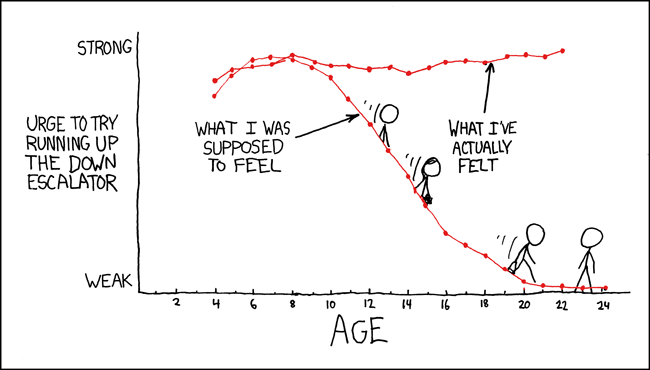
\includegraphics[width=.45\textwidth]{figures/escalators.png}}
  \end{figure}

When you print tables, it's good style to highlight the best results in bold. Also use the \textsc{booktabs} package for nicely formatted tables, as explained in the previous section on \LaTeX{} advice. (That's not a must, but it will simply look much nicer!)                    % evaluation
\chapter{Concluding Remarks}\label{chap:conclusion}

If you wish, you may also name that section \emph{``Conclusion and Future Work''}, though it might not be a perfect choice to have a section named ``A \& B'' if it has subsections ``A'' and ``B''. Also note that you don't necessarily have to use these subsections; that also depends on how much content you have in each. (E.g., having a section header might be odd if it contains just three lines.)


\section{Conclusion}

This section usually summarizes the entire paper including the conclusions drawn, e.g., did the developed techniques work? Maybe add why or why not. Also don't hold back on limitations of your work; it shows that you understood what you have done. And science isn't about claiming how great something is, but about objectively testing hypotheses. Also note that every single scientific paper has such a section, so you can check out many examples, preferably at top-tier venues, e.g., by your supervisor(s).


\section{Future Work}

On top of that, you could discuss future work (and make clear why that is future work, i.e., by which observations did they get justified?).

Note that future work in scientific papers is often not mentioned at all or just in a very few sentences within the conclusion. That should not stop you from putting some effort in. This will (also) show the examiner(s)/supervisor(s) how well you understood the topic or how engaged you are.
                    % conclusion

\appendix
\chapter{Appendix: Explanation on Appendices}\label{chap:appendix1}

You may use appendices to provide additional information that is in principle relevant to your work, though you don't want \emph{every reader} to look at the entire material, but only those interested.

There are many cases where an appendix may make sense. For example:
\begin{itemize}
  \item You developed various variants of some algorithm, but you only describe one of them in the main body, since the different variants are not that different.
  \item You may have conducted an extensive empirical analysis, yet you don't want to provide \emph{all} results. So you focus on the most relevant results in the main body of your work to get the message across. Yet you present the remaining and complete results here for the more interested reader.
  \item You developed a model of some sort. In your work, you explained an excerpt of the model. You also used mathematical syntax for this. Here, you can (if you wish) provide the actual model as you provided it in probably some textfile. Note that you don't have to do this, as artifacts can be submitted separately. Consult your supervisor in such a case.
  \item You could also provide a list of figures and/or list of tables in here (via the commands \verb!\listoffigures! and \verb!\listoftables!, respectively). Do this only if you think that this is beneficial for your work. If you want to include it, you can of course also provide it right after the table of contents. You might want to make this dependent on how many people you think are interested in this.
\end{itemize}
                    % appendix 1
\chapter{Appendix: Explanation on Page Borders}\label{chap:appendix2}

What you find here is an explanation of why the border width keeps flipping from left to right -- which you might have spotted and wondered why that's the case.

Firstly, that is \emph{intended} and thus correct, so there is no reason to worry about this. The reason is that this document is configured as a two-sided book, which means:
\begin{compactitem}
  \item We assume the document will be printed out,
  \item that this will be done in a two-sided mode (i.e., the document will be printed on both sides of each page), and
  \item that the bookbinding will be in the middle, just like in every book.
\end{compactitem}

When you open the book, there are three borders of equal size~$n$. This however requires that even pages have a border of $n$ on their left and $\frac{n}{2}$ on their right, and odd pages have a border of $\frac{n}{2}$ on their left and $n$ on their right. This is illustrated in Figure~\ref{fig:pageBorders}.

\begin{figure}[h]
  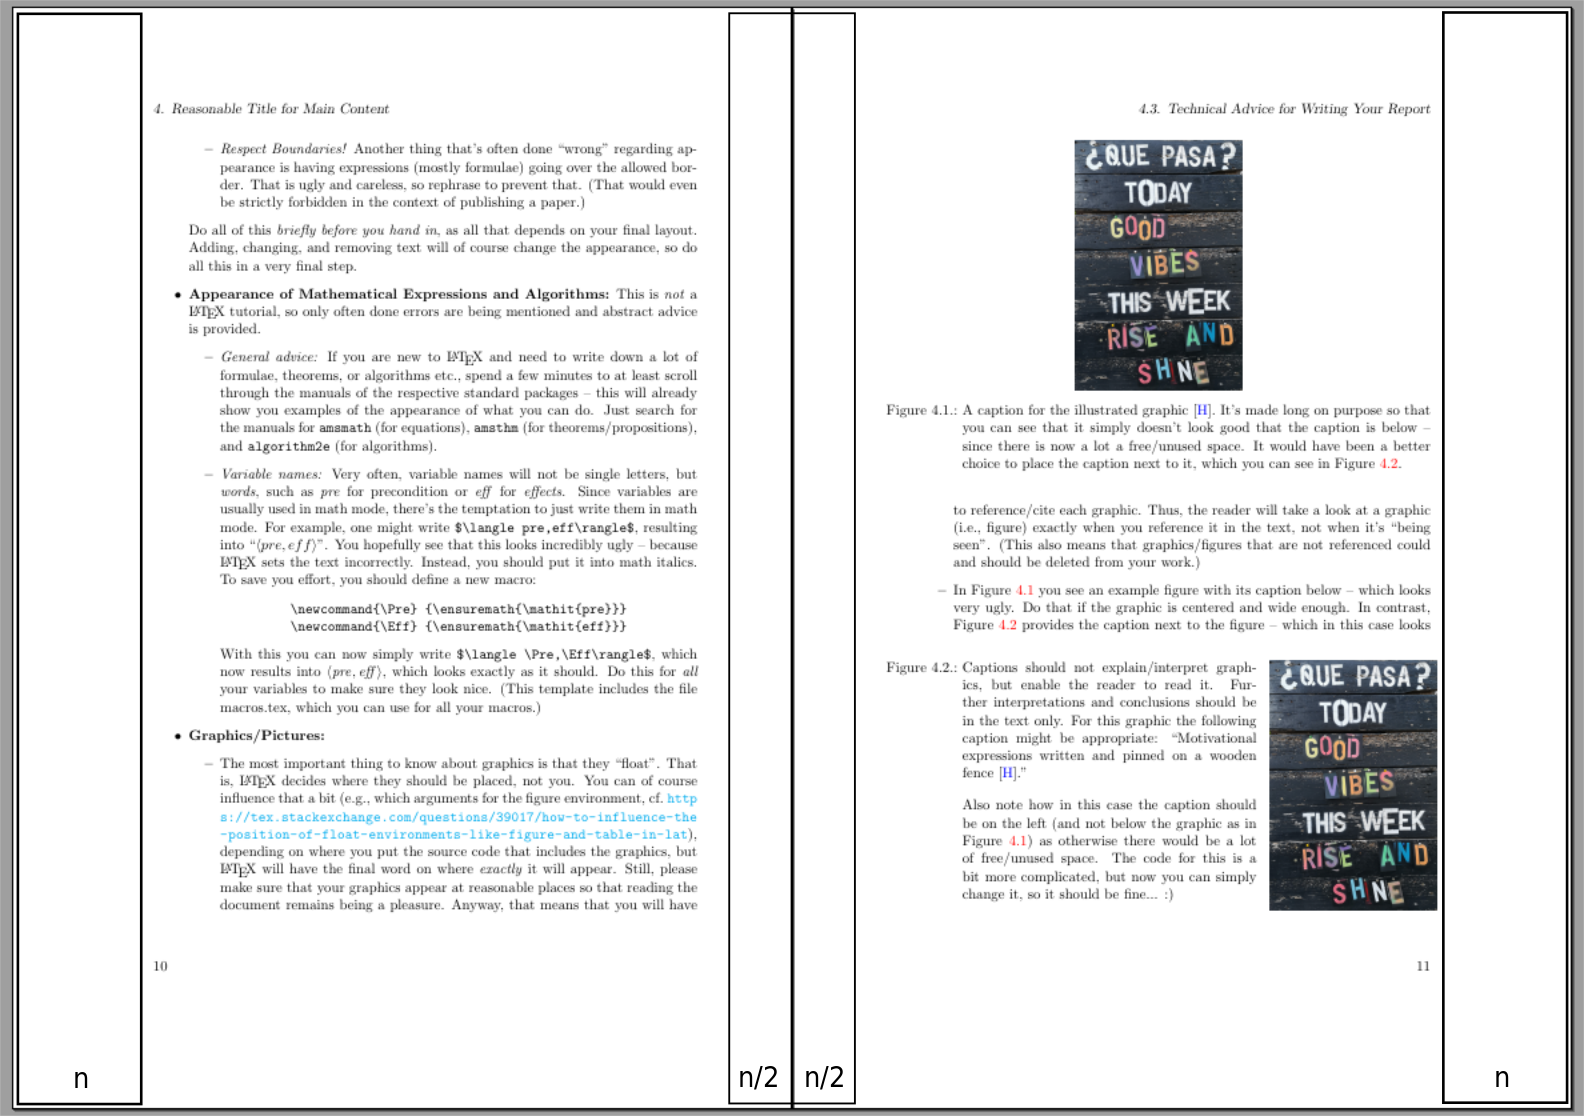
\includegraphics[width=.55\textwidth]{figures/borders--annotated}
  \caption{Illustration showing why page borders flip.\label{fig:pageBorders}}
\end{figure}%

                    % appendix 2


% literature
\bibliographystyle{anuthesis} % or plainnat or whatever
\cleardoublepage\phantomsection
% see https://tex.stackexchange.com/questions/60556/link-to-bibliography-in-the-toc-fails
\bibliography{bib}
\end{document}
